% This is the Reed College LaTeX thesis template. Most of the work
% for the document class was done by Sam Noble (SN), as well as this
% template. Later comments etc. by Ben Salzberg (BTS). Additional
% restructuring and APA support by Jess Youngberg (JY).
% Your comments and suggestions are more than welcome; please email
% them to cus@reed.edu
%
% See http://web.reed.edu/cis/help/latex.html for help. There are a
% great bunch of help pages there, with notes on
% getting started, bibtex, etc. Go there and read it if you're not
% already familiar with LaTeX.
%
% Any line that starts with a percent symbol is a comment.
% They won't show up in the document, and are useful for notes
% to yourself and explaining commands.
% Commenting also removes a line from the document;
% very handy for troubleshooting problems. -BTS

% As far as I know, this follows the requirements laid out in
% the 2002-2003 Senior Handbook. Ask a librarian to check the
% document before binding. -SN

%%
%% Preamble
%%
% \documentclass{<something>} must begin each LaTeX document
\documentclass[12pt,twoside]{reedthesis}
% Packages are extensions to the basic LaTeX functions. Whatever you
% want to typeset, there is probably a package out there for it.
% Chemistry (chemtex), screenplays, you name it.
% Check out CTAN to see: http://www.ctan.org/
%%
\usepackage{graphicx,latexsym}
\usepackage{amsmath}
\usepackage{amssymb,amsthm}
\usepackage{longtable,booktabs,setspace}
\usepackage{chemarr} %% Useful for one reaction arrow, useless if you're not a chem major
\usepackage[hyphens]{url}
% Added by CII
\usepackage{hyperref}
\usepackage{lmodern}
\usepackage{float}
\floatplacement{figure}{H}
% End of CII addition
\usepackage{rotating}

% Next line commented out by CII
%%% \usepackage{natbib}
% Comment out the natbib line above and uncomment the following two lines to use the new
% biblatex-chicago style, for Chicago A. Also make some changes at the end where the
% bibliography is included.
%\usepackage{biblatex-chicago}
%\bibliography{thesis}


% Added by CII (Thanks, Hadley!)
% Use ref for internal links
\renewcommand{\hyperref}[2][???]{\autoref{#1}}
\def\chapterautorefname{Chapter}
\def\sectionautorefname{Section}
\def\subsectionautorefname{Subsection}
% End of CII addition

% Added by CII
\usepackage{caption}
\captionsetup{width=5in}
% End of CII addition

% \usepackage{times} % other fonts are available like times, bookman, charter, palatino

% Syntax highlighting #22
  \usepackage{color}
  \usepackage{fancyvrb}
  \newcommand{\VerbBar}{|}
  \newcommand{\VERB}{\Verb[commandchars=\\\{\}]}
  \DefineVerbatimEnvironment{Highlighting}{Verbatim}{commandchars=\\\{\}}
  % Add ',fontsize=\small' for more characters per line
  \usepackage{framed}
  \definecolor{shadecolor}{RGB}{248,248,248}
  \newenvironment{Shaded}{\begin{snugshade}}{\end{snugshade}}
  \newcommand{\AlertTok}[1]{\textcolor[rgb]{0.94,0.16,0.16}{#1}}
  \newcommand{\AnnotationTok}[1]{\textcolor[rgb]{0.56,0.35,0.01}{\textbf{\textit{#1}}}}
  \newcommand{\AttributeTok}[1]{\textcolor[rgb]{0.77,0.63,0.00}{#1}}
  \newcommand{\BaseNTok}[1]{\textcolor[rgb]{0.00,0.00,0.81}{#1}}
  \newcommand{\BuiltInTok}[1]{#1}
  \newcommand{\CharTok}[1]{\textcolor[rgb]{0.31,0.60,0.02}{#1}}
  \newcommand{\CommentTok}[1]{\textcolor[rgb]{0.56,0.35,0.01}{\textit{#1}}}
  \newcommand{\CommentVarTok}[1]{\textcolor[rgb]{0.56,0.35,0.01}{\textbf{\textit{#1}}}}
  \newcommand{\ConstantTok}[1]{\textcolor[rgb]{0.00,0.00,0.00}{#1}}
  \newcommand{\ControlFlowTok}[1]{\textcolor[rgb]{0.13,0.29,0.53}{\textbf{#1}}}
  \newcommand{\DataTypeTok}[1]{\textcolor[rgb]{0.13,0.29,0.53}{#1}}
  \newcommand{\DecValTok}[1]{\textcolor[rgb]{0.00,0.00,0.81}{#1}}
  \newcommand{\DocumentationTok}[1]{\textcolor[rgb]{0.56,0.35,0.01}{\textbf{\textit{#1}}}}
  \newcommand{\ErrorTok}[1]{\textcolor[rgb]{0.64,0.00,0.00}{\textbf{#1}}}
  \newcommand{\ExtensionTok}[1]{#1}
  \newcommand{\FloatTok}[1]{\textcolor[rgb]{0.00,0.00,0.81}{#1}}
  \newcommand{\FunctionTok}[1]{\textcolor[rgb]{0.00,0.00,0.00}{#1}}
  \newcommand{\ImportTok}[1]{#1}
  \newcommand{\InformationTok}[1]{\textcolor[rgb]{0.56,0.35,0.01}{\textbf{\textit{#1}}}}
  \newcommand{\KeywordTok}[1]{\textcolor[rgb]{0.13,0.29,0.53}{\textbf{#1}}}
  \newcommand{\NormalTok}[1]{#1}
  \newcommand{\OperatorTok}[1]{\textcolor[rgb]{0.81,0.36,0.00}{\textbf{#1}}}
  \newcommand{\OtherTok}[1]{\textcolor[rgb]{0.56,0.35,0.01}{#1}}
  \newcommand{\PreprocessorTok}[1]{\textcolor[rgb]{0.56,0.35,0.01}{\textit{#1}}}
  \newcommand{\RegionMarkerTok}[1]{#1}
  \newcommand{\SpecialCharTok}[1]{\textcolor[rgb]{0.00,0.00,0.00}{#1}}
  \newcommand{\SpecialStringTok}[1]{\textcolor[rgb]{0.31,0.60,0.02}{#1}}
  \newcommand{\StringTok}[1]{\textcolor[rgb]{0.31,0.60,0.02}{#1}}
  \newcommand{\VariableTok}[1]{\textcolor[rgb]{0.00,0.00,0.00}{#1}}
  \newcommand{\VerbatimStringTok}[1]{\textcolor[rgb]{0.31,0.60,0.02}{#1}}
  \newcommand{\WarningTok}[1]{\textcolor[rgb]{0.56,0.35,0.01}{\textbf{\textit{#1}}}}

% To pass between YAML and LaTeX the dollar signs are added by CII
\title{Spatio temporal analysis of extreme wind velocities for infrastructure desing. Case study Colombia}
\author{Alexys Herleym Rodríguez Avellaneda}
% The month and year that you submit your FINAL draft TO THE LIBRARY (May or December)
\date{Jan 2020}
\division{Instituto for Geoinformatics - IFGI}
\advisor{Dr.~Edzer Pebesma}
\institution{University of Münster}
\degree{Master of Science in Geospatial Technologies}
%If you have two advisors for some reason, you can use the following
% Uncommented out by CII
\altadvisor{Dr.~Juan C. Reyes}
% End of CII addition

%%% Remember to use the correct department!
\department{}
% if you're writing a thesis in an interdisciplinary major,
% uncomment the line below and change the text as appropriate.
% check the Senior Handbook if unsure.
%\thedivisionof{The Established Interdisciplinary Committee for}
% if you want the approval page to say "Approved for the Committee",
% uncomment the next line
%\approvedforthe{Committee}

% Added by CII
%%% Copied from knitr
%% maxwidth is the original width if it's less than linewidth
%% otherwise use linewidth (to make sure the graphics do not exceed the margin)
\makeatletter
\def\maxwidth{ %
  \ifdim\Gin@nat@width>\linewidth
    \linewidth
  \else
    \Gin@nat@width
  \fi
}
\makeatother

\renewcommand{\contentsname}{Table of Contents}
% End of CII addition

\setlength{\parskip}{0pt}

% Added by CII

\providecommand{\tightlist}{%
  \setlength{\itemsep}{0pt}\setlength{\parskip}{0pt}}

\Acknowledgements{
I want to thank a few people.
}

\Dedication{
You can have a dedication here if you wish.
}

\Preface{
This is an example of a thesis setup to use the reed thesis document class
(for LaTeX) and the R bookdown package, in general.
}

\Abstract{
The preface pretty much says it all.

\par

Second paragraph of abstract starts here.
}

% End of CII addition
%%
%% End Preamble
%%
%
\begin{document}

% Everything below added by CII
  \maketitle

\frontmatter % this stuff will be roman-numbered
\pagestyle{empty} % this removes page numbers from the frontmatter
  \begin{acknowledgements}
    I want to thank a few people.
  \end{acknowledgements}
  \begin{preface}
    This is an example of a thesis setup to use the reed thesis document class
    (for LaTeX) and the R bookdown package, in general.
  \end{preface}
  \hypersetup{linkcolor=black}
  \setcounter{tocdepth}{2}
  \tableofcontents

  \listoftables

  \listoffigures
  \begin{abstract}
    The preface pretty much says it all.
    
    \par
    
    Second paragraph of abstract starts here.
  \end{abstract}
  \begin{dedication}
    You can have a dedication here if you wish.
  \end{dedication}
\mainmatter % here the regular arabic numbering starts
\pagestyle{fancyplain} % turns page numbering back on

\hypertarget{introduction}{%
\chapter*{Introduction}\label{introduction}}
\addcontentsline{toc}{chapter}{Introduction}

Placeholder

\hypertarget{rmd-data}{%
\chapter{Data}\label{rmd-data}}

Placeholder

\hypertarget{ideam}{%
\section{IDEAM}\label{ideam}}

\hypertarget{isd}{%
\section{ISD}\label{isd}}

\hypertarget{era5}{%
\section{ERA5}\label{era5}}

\hypertarget{section}{%
\section{}\label{section}}

\hypertarget{data-download-and-organization}{%
\section{Data Download and Organization}\label{data-download-and-organization}}

\hypertarget{data-standarzation}{%
\section{Data Standarzation}\label{data-standarzation}}

\hypertarget{rmd-thefra}{%
\chapter{Theoretical Framework}\label{rmd-thefra}}

\hypertarget{probability-concepts}{%
\section{Probability Concepts}\label{probability-concepts}}

Poisson process is an stochastic method that relies in the concepts of probability distributions. The main functions related to probability for extreme value analysis will be described below.

\hypertarget{probability-density-function---pdf}{%
\subsection{\texorpdfstring{Probability Density Function - \emph{pdf}}{Probability Density Function - pdf}}\label{probability-density-function---pdf}}

Pdf defines the probability that a continuos variable falls between two points, this is, in \emph{pdf} the proability is related to the area below the curve (integral) between two points, as for continuos probability distributions the probability at a single point is zero. The term density is directly related to the probability of a portion of the curve, if the density function has high values the probability will be greater in comparison with the same portion of curve for low values.

\[
\int_a^b f(x)dx = Pr[a \leq X \leq b]
\]

Equation \eqref{eq:gumbelpdf} is the Gumbel \emph{pdf}.
\begin{equation}
  \mathrm{
          f(x)=\frac{1}{\beta}
          \exp\left\{
            -\frac{x-\mu}{\beta}
          \right\}
          \exp\left\{
            -\exp\left\{
              -\left(
                \frac{x-\mu}{\beta}
              \right)
            \right\}
          \right\},
          \quad -\infty < x < \infty
         }
  \label{eq:gumbelpdf}
\end{equation}
where \(\exp\left\{.\right\} \mapsto \mathrm{e}^{\left\{.\right\}}\), \(\beta\) is the scale parameter, and \(\mu\) is the location parameter. Location (\(\mu\)) has the effect to shift the \emph{pdf} to left or right along `x' axis, thus, if location value is changed the effect is a movement of \emph{pdf} to the left (small value for location), or to the right (big value for location). Scale has the effect to stretch (\(\beta > 1\)) of compress (\(0 < \beta< 1\)) the \emph{pdf}, if scale parameter is close to zero the pdf approaches a spike.

Figure \ref{fig:plotgumbelpdffunction} shows \emph{pdf} with location (\(\mu\)) = 100 and scale (\(\beta\)) = 40, using equation \eqref{eq:gumbelpdf}.

\footnotesize
\begin{Shaded}
\begin{Highlighting}[]
\NormalTok{location =}\StringTok{ }\DecValTok{100}
\NormalTok{scale =}\StringTok{ }\DecValTok{40}
\NormalTok{.x <-}\StringTok{ }\KeywordTok{seq}\NormalTok{(}\DecValTok{0}\NormalTok{, }\DecValTok{300}\NormalTok{, }\DataTypeTok{length.out=}\DecValTok{1000}\NormalTok{)}
\NormalTok{pdfG <-}\StringTok{ }\ControlFlowTok{function}\NormalTok{(x) \{}
  \DecValTok{1}\OperatorTok{/}\NormalTok{location }\OperatorTok{*}\KeywordTok{exp}\NormalTok{(}\OperatorTok{-}\NormalTok{(x}\OperatorTok{-}\NormalTok{location)}\OperatorTok{/}\NormalTok{scale)}\OperatorTok{*}\KeywordTok{exp}\NormalTok{(}\OperatorTok{-}\KeywordTok{exp}\NormalTok{(}\OperatorTok{-}\NormalTok{(x}\OperatorTok{-}\NormalTok{location)}\OperatorTok{/}\NormalTok{scale))}
\NormalTok{  \}}
\NormalTok{.y =}\StringTok{ }\KeywordTok{pdfG}\NormalTok{(.x)}
\KeywordTok{plot}\NormalTok{(.x, .y, }\DataTypeTok{col=}\StringTok{"green"}\NormalTok{, }\DataTypeTok{lty=}\DecValTok{4}\NormalTok{, }
     \DataTypeTok{xlab=}\StringTok{"Velocities Km/h"}\NormalTok{, }\DataTypeTok{ylab=}\StringTok{"Density Function - Gumbel Distribution"}\NormalTok{, }
     \DataTypeTok{main=}\KeywordTok{paste}\NormalTok{(}\StringTok{"Gumbel - Density Function Gumbel Distribution}\CharTok{\textbackslash{}n}\StringTok{"}\NormalTok{, }\StringTok{"Location="}\NormalTok{, }
     \KeywordTok{round}\NormalTok{(location,}\DecValTok{2}\NormalTok{), }\StringTok{" Scale="}\NormalTok{, }\KeywordTok{round}\NormalTok{(scale,}\DecValTok{2}\NormalTok{)), }\DataTypeTok{type=}\StringTok{"l"}\NormalTok{, }
     \DataTypeTok{cex.axis =} \FloatTok{0.5}\NormalTok{, }\DataTypeTok{cex.lab=} \FloatTok{0.6}\NormalTok{, }\DataTypeTok{cex.main=}\FloatTok{0.7}\NormalTok{, }\DataTypeTok{cex.sub=}\FloatTok{0.6}\NormalTok{)}
\end{Highlighting}
\end{Shaded}
\begin{figure}
\centering
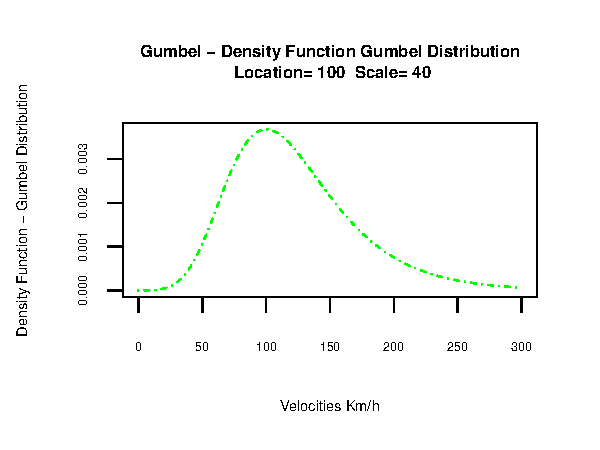
\includegraphics{thesis_files/figure-latex/plotgumbelpdffunction-1.pdf}
\caption{\label{fig:plotgumbelpdffunction}Gumbel pdf}
\end{figure}
\normalsize

Figure \ref{fig:plotgumbelpdf} shows \emph{pdf} with location (\(\mu\)) = 100 and scale (\(\beta\)) = 40, using function \texttt{dgumbel} of the package \texttt{RcmdrMisc}

\footnotesize
\begin{Shaded}
\begin{Highlighting}[]
\NormalTok{location =}\StringTok{ }\DecValTok{100}
\NormalTok{scale =}\StringTok{ }\DecValTok{40}
\NormalTok{.x <-}\StringTok{ }\KeywordTok{seq}\NormalTok{(}\DecValTok{0}\NormalTok{, }\DecValTok{300}\NormalTok{, }\DataTypeTok{length.out=}\DecValTok{1000}\NormalTok{)}
\NormalTok{dfG =}\StringTok{ }\KeywordTok{dgumbel}\NormalTok{(.x, }\DataTypeTok{location=}\NormalTok{location, }\DataTypeTok{scale=}\NormalTok{scale)}
\KeywordTok{plot}\NormalTok{(.x, dfG, }\DataTypeTok{col=}\StringTok{"red"}\NormalTok{, }\DataTypeTok{lty=}\DecValTok{4}\NormalTok{, }
     \DataTypeTok{xlab=}\StringTok{"Velocities Km/h"}\NormalTok{, }\DataTypeTok{ylab=}\StringTok{"Density Function - Gumbel Distribution"}\NormalTok{, }
     \DataTypeTok{main=}\KeywordTok{paste}\NormalTok{(}\StringTok{"Gumbel - Density Function Gumbel Distribution}\CharTok{\textbackslash{}n}\StringTok{"}\NormalTok{, }\StringTok{"Location="}\NormalTok{, }
     \KeywordTok{round}\NormalTok{(location,}\DecValTok{2}\NormalTok{), }\StringTok{" Scale="}\NormalTok{, }\KeywordTok{round}\NormalTok{(scale,}\DecValTok{2}\NormalTok{)), }\DataTypeTok{type=}\StringTok{"l"}\NormalTok{, }
     \DataTypeTok{cex.axis =} \FloatTok{0.5}\NormalTok{, }\DataTypeTok{cex.lab=} \FloatTok{0.6}\NormalTok{, }\DataTypeTok{cex.main=}\FloatTok{0.7}\NormalTok{, }\DataTypeTok{cex.sub=}\FloatTok{0.6}\NormalTok{)}
\end{Highlighting}
\end{Shaded}
\begin{figure}
\centering
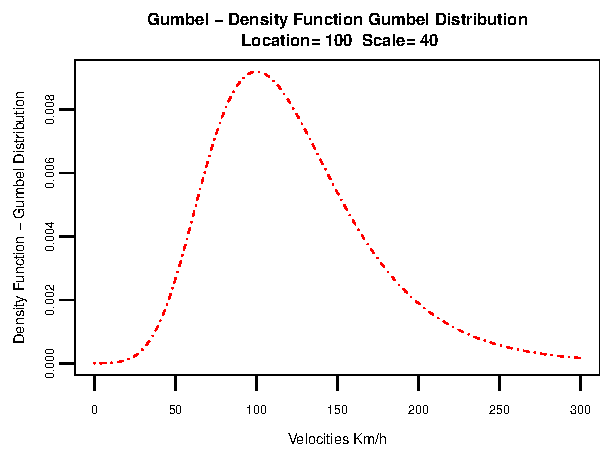
\includegraphics{thesis_files/figure-latex/plotgumbelpdf-1.pdf}
\caption{\label{fig:plotgumbelpdf}Gumbel pdf - dgumbel function}
\end{figure}
\normalsize

\hypertarget{cumulative-distribution-funtcion---cdf}{%
\subsection{\texorpdfstring{Cumulative Distribution Funtcion - \emph{cdf}}{Cumulative Distribution Funtcion - cdf}}\label{cumulative-distribution-funtcion---cdf}}

\emph{Cdf} is the probability of taking a value less than or equal to x. That is

\[
F(x) = Pr[X < x] = \alpha
\]
For a continuous variable, \emph{cdf} can be expressed as the integral of its \emph{pdf}.
\[
F(x) = \int_{-\infty}^x f(x)dx
\]

Equation \eqref{eq:gumbelcdf} is the Gumbel \emph{cdf}.
\begin{equation}
\mathrm{
        F(x) = \exp\left\{-\exp\left[-\left(\frac{x-\mu}{\beta}\right)\right]\right\}, 
        \quad -\infty < x < \infty
        }
  \label{eq:gumbelcdf}
\end{equation}
Figure \ref{fig:plotgumbelcdffunction} shows Gumbel \emph{cdf} with location (\(\mu\)) = 100 and scale (\(\beta\)) = 40, using equation \eqref{eq:gumbelcdf}. As previously done with \emph{pdf}, similar result can be achieved using function \texttt{pgumbel} of package \texttt{RcmdrMisc}.

\footnotesize
\begin{Shaded}
\begin{Highlighting}[]
\NormalTok{location =}\StringTok{ }\DecValTok{100}
\NormalTok{scale =}\StringTok{ }\DecValTok{40}
\NormalTok{.x <-}\StringTok{ }\KeywordTok{seq}\NormalTok{(}\DecValTok{0}\NormalTok{, }\DecValTok{300}\NormalTok{, }\DataTypeTok{length.out=}\DecValTok{1000}\NormalTok{)}
\NormalTok{cdfG <-}\StringTok{ }\ControlFlowTok{function}\NormalTok{(x) \{}
  \KeywordTok{exp}\NormalTok{(}\OperatorTok{-}\KeywordTok{exp}\NormalTok{(}\OperatorTok{-}\NormalTok{(x}\OperatorTok{-}\NormalTok{location)}\OperatorTok{/}\NormalTok{scale))}
\NormalTok{  \}}
\NormalTok{.y =}\StringTok{ }\KeywordTok{cdfG}\NormalTok{(.x)}
\KeywordTok{plot}\NormalTok{(.x, .y, }\DataTypeTok{col=}\StringTok{"green"}\NormalTok{, }\DataTypeTok{lty=}\DecValTok{4}\NormalTok{, }
     \DataTypeTok{xlab=}\StringTok{"Velocities Km/h"}\NormalTok{, }\DataTypeTok{ylab=}\StringTok{"Probability"}\NormalTok{, }
     \DataTypeTok{main=}\KeywordTok{paste}\NormalTok{(}\StringTok{"Gumbel - Cumulative Distribution Function}\CharTok{\textbackslash{}n}\StringTok{"}\NormalTok{, }\StringTok{"Location="}\NormalTok{, }
     \KeywordTok{round}\NormalTok{(location,}\DecValTok{2}\NormalTok{), }\StringTok{" Scale="}\NormalTok{, }\KeywordTok{round}\NormalTok{(scale,}\DecValTok{2}\NormalTok{)), }\DataTypeTok{type=}\StringTok{"l"}\NormalTok{, }
     \DataTypeTok{cex.axis =} \FloatTok{0.5}\NormalTok{, }\DataTypeTok{cex.lab=} \FloatTok{0.6}\NormalTok{, }\DataTypeTok{cex.main=}\FloatTok{0.7}\NormalTok{, }\DataTypeTok{cex.sub=}\FloatTok{0.6}\NormalTok{)}
\end{Highlighting}
\end{Shaded}
\begin{figure}
\centering
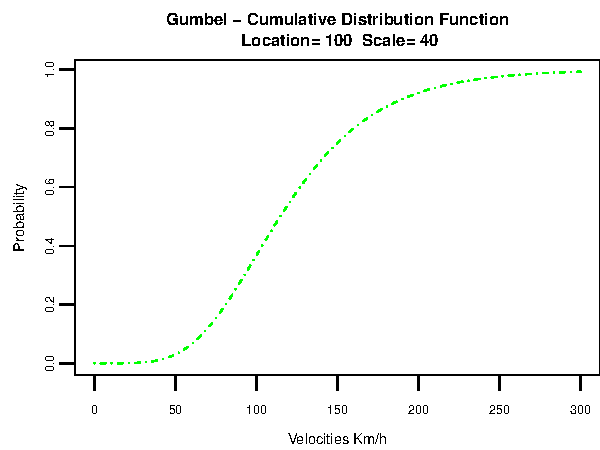
\includegraphics{thesis_files/figure-latex/plotgumbelcdffunction-1.pdf}
\caption{\label{fig:plotgumbelcdffunction}Gumbel cdf}
\end{figure}
\normalsize

\hypertarget{percent-point-function---ppf}{%
\subsection{\texorpdfstring{Percent Point Function - \emph{ppf}}{Percent Point Function - ppf}}\label{percent-point-function---ppf}}

\emph{Ppf} is the inverse of \emph{cdf}, also called the \emph{quantile} function. This is, from a specific probability get the corresponding value x of the variable.

\[
x = G(\alpha) = G(F(x))
\]
Equation \eqref{eq:gumbelppf} is the Gumbel \emph{ppf}.
\begin{equation}
\mathrm{
        G(\alpha) = \mu-\beta ln(-ln(\alpha))
        \quad 0 < \alpha < 1
        }
  \label{eq:gumbelppf}
\end{equation}
Figure \ref{fig:plotgumbelppffunction} shows Gumbel \emph{ppf}, using equation \eqref{eq:gumbelppf}. Similar result can be achieved using function \texttt{qgumbel} of package \texttt{RcmdrMisc}.

\footnotesize
\begin{Shaded}
\begin{Highlighting}[]
\NormalTok{location =}\StringTok{ }\DecValTok{100}
\NormalTok{scale =}\StringTok{ }\DecValTok{40}
\NormalTok{.x <-}\StringTok{ }\KeywordTok{seq}\NormalTok{(}\DecValTok{0}\NormalTok{, }\DecValTok{1}\NormalTok{, }\DataTypeTok{length.out=}\DecValTok{1000}\NormalTok{)}
\NormalTok{ppfG <-}\StringTok{ }\ControlFlowTok{function}\NormalTok{(x) \{}
\NormalTok{  location }\OperatorTok{-}\StringTok{ }\NormalTok{(scale}\OperatorTok{*}\KeywordTok{log}\NormalTok{(}\OperatorTok{-}\KeywordTok{log}\NormalTok{(x)))}
\NormalTok{  \}}
\NormalTok{.y =}\StringTok{ }\KeywordTok{ppfG}\NormalTok{(.x)}
\KeywordTok{plot}\NormalTok{(.x, .y, }\DataTypeTok{col=}\StringTok{"green"}\NormalTok{, }\DataTypeTok{lty=}\DecValTok{4}\NormalTok{, }
     \DataTypeTok{ylab=}\StringTok{"Velocities Km/h"}\NormalTok{, }\DataTypeTok{xlab=}\StringTok{"Probability"}\NormalTok{, }
     \DataTypeTok{main=}\KeywordTok{paste}\NormalTok{(}\StringTok{"Gumbel - Percent Point Function}\CharTok{\textbackslash{}n}\StringTok{"}\NormalTok{, }\StringTok{"Location="}\NormalTok{, }
     \KeywordTok{round}\NormalTok{(location,}\DecValTok{2}\NormalTok{), }\StringTok{" Scale="}\NormalTok{, }\KeywordTok{round}\NormalTok{(scale,}\DecValTok{2}\NormalTok{)), }\DataTypeTok{type=}\StringTok{"l"}\NormalTok{, }
     \DataTypeTok{cex.axis =} \FloatTok{0.5}\NormalTok{, }\DataTypeTok{cex.lab=} \FloatTok{0.6}\NormalTok{, }\DataTypeTok{cex.main=}\FloatTok{0.7}\NormalTok{, }\DataTypeTok{cex.sub=}\FloatTok{0.6}\NormalTok{)}
\end{Highlighting}
\end{Shaded}
\begin{figure}
\centering
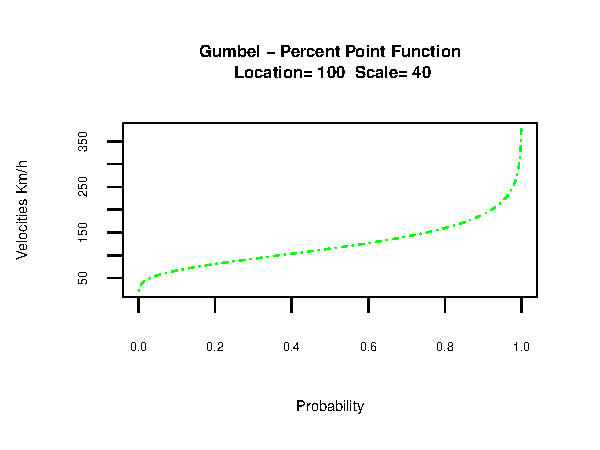
\includegraphics{thesis_files/figure-latex/plotgumbelppffunction-1.pdf}
\caption{\label{fig:plotgumbelppffunction}Gumbel cdf}
\end{figure}
\normalsize

\hypertarget{hazard-function---hf}{%
\subsection{\texorpdfstring{Hazard Function - \emph{hf}}{Hazard Function - hf}}\label{hazard-function---hf}}

Using \(S(x) = 1 - F(x)\) as survival function -\emph{sf}, the probability that a variable takes a value greather than x \(S(x) = Pr[X > x] = 1 - F(x)\), the \emph{hf} is the ratio between \emph{pdf} and \emph{sf}.

\[
h(x) = \frac{f(x)}{S(x)} = \frac{f(x)}{1-F(x)}
\]
Equation \eqref{eq:gumbelhf} is the Gumbel \emph{ppf}.

Figure \ref{fig:plotgumbelhfffunction} shows Gumbel \emph{hf}, using equation \eqref{eq:gumbelhf}.

\footnotesize
\begin{Shaded}
\begin{Highlighting}[]
\NormalTok{location =}\StringTok{ }\DecValTok{100}
\NormalTok{scale =}\StringTok{ }\DecValTok{40}
\NormalTok{.x <-}\StringTok{ }\KeywordTok{seq}\NormalTok{(}\DecValTok{0}\NormalTok{, }\DecValTok{300}\NormalTok{, }\DataTypeTok{length.out=}\DecValTok{1000}\NormalTok{)}
\NormalTok{hfG <-}\StringTok{ }\ControlFlowTok{function}\NormalTok{(x) \{}
\NormalTok{  (}\DecValTok{1}\OperatorTok{/}\NormalTok{scale)}\OperatorTok{*}\NormalTok{(}\KeywordTok{exp}\NormalTok{(}\OperatorTok{-}\NormalTok{(x}\OperatorTok{-}\NormalTok{location)}\OperatorTok{/}\NormalTok{scale))}\OperatorTok{/}\NormalTok{(}\KeywordTok{exp}\NormalTok{(}\KeywordTok{exp}\NormalTok{(}\OperatorTok{-}\NormalTok{(x}\OperatorTok{-}\NormalTok{location)}\OperatorTok{/}\NormalTok{scale))}\OperatorTok{-}\DecValTok{1}\NormalTok{)}
\NormalTok{  \}}
\NormalTok{.y =}\StringTok{ }\KeywordTok{hfG}\NormalTok{(.x)}
\KeywordTok{plot}\NormalTok{(.x, .y, }\DataTypeTok{col=}\StringTok{"green"}\NormalTok{, }\DataTypeTok{lty=}\DecValTok{4}\NormalTok{, }
     \DataTypeTok{xlab=}\StringTok{"Velocities Km/h"}\NormalTok{, }\DataTypeTok{ylab=}\StringTok{"Hazard"}\NormalTok{, }
     \DataTypeTok{main=}\KeywordTok{paste}\NormalTok{(}\StringTok{"Gumbel - Hazard Function}\CharTok{\textbackslash{}n}\StringTok{"}\NormalTok{, }\StringTok{"Location="}\NormalTok{, }
     \KeywordTok{round}\NormalTok{(location,}\DecValTok{2}\NormalTok{), }\StringTok{" Scale="}\NormalTok{, }\KeywordTok{round}\NormalTok{(scale,}\DecValTok{2}\NormalTok{)), }\DataTypeTok{type=}\StringTok{"l"}\NormalTok{, }
     \DataTypeTok{cex.axis =} \FloatTok{0.5}\NormalTok{, }\DataTypeTok{cex.lab=} \FloatTok{0.6}\NormalTok{, }\DataTypeTok{cex.main=}\FloatTok{0.7}\NormalTok{, }\DataTypeTok{cex.sub=}\FloatTok{0.6}\NormalTok{)}
\end{Highlighting}
\end{Shaded}
\begin{figure}
\centering
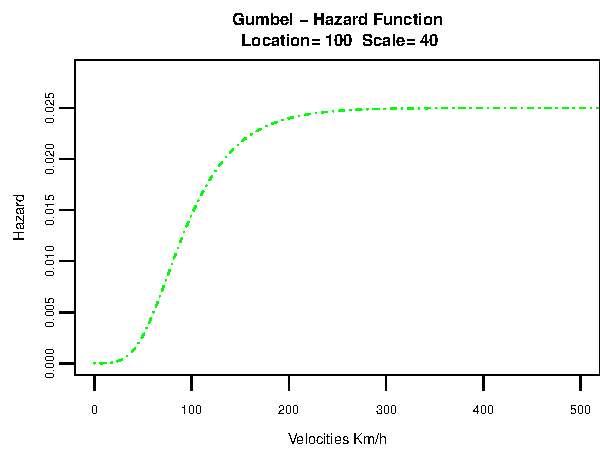
\includegraphics{thesis_files/figure-latex/plotgumbelhffunction-1.pdf}
\caption{\label{fig:plotgumbelhffunction}Gumbel cdf}
\end{figure}
\normalsize

\hypertarget{cumulative-hazard-function}{%
\subsection{Cumulative Hazard Function}\label{cumulative-hazard-function}}

\[
\sum_{j=1}^n (\delta\theta_j)^2 \leq {{\beta_i^2}\over{\delta_i^2 + \rho_i^2}}
\left[ 2\rho_i^2 + {\delta_i^2\beta_i^2\over{\delta_i^2 + \rho_i^2}} \right] \equiv \omega_i^2
\]
\begin{equation}
  \mathrm{\sum_{j=1}^n (\delta\theta_j)^2 \leq {{\beta_i^2}\over{\delta_i^2 + \rho_i^2}}
\left[ 2\rho_i^2 + {\delta_i^2\beta_i^2\over{\delta_i^2 + \rho_i^2}} \right] \equiv \omega_i^2}
  \label{eq:gumbelpdf2}
\end{equation}
We can reference this combustion of glucose reaction via Equation \eqref{eq:gumbelpdf}.

\[\sum_{j=1}^n (\delta\theta_j)^2 \leq {{\beta_i^2}\over{\delta_i^2 + \rho_i^2}}
\left[ 2\rho_i^2 + {\delta_i^2\beta_i^2\over{\delta_i^2 + \rho_i^2}} \right] \equiv \omega_i^2
\]

\TeX~is the best way to typeset mathematics. Donald Knuth designed \TeX~when he got frustrated at how long it was taking the typesetters to finish his book, which contained a lot of mathematics. One nice feature of \emph{R Markdown} is its ability to read LaTeX code directly.

If you are doing a thesis that will involve lots of math, you will want to read the following section which has been commented out. If you're not going to use math, skip over or delete this next commented section.

\[\sum_{j=1}^n (\delta\theta_j)^2 \leq {{\beta_i^2}\over{\delta_i^2 + \rho_i^2}}
\left[ 2\rho_i^2 + {\delta_i^2\beta_i^2\over{\delta_i^2 + \rho_i^2}} \right] \equiv \omega_i^2
\]

From Informational Dynamics, we have the following (Dave Braden):

After \emph{n} such encounters the posterior density for \(\theta\) is

\[
\pi(\theta|X_1< y_1,\dots,X_n<y_n) \varpropto \pi(\theta) \prod_{i=1}^n\int_{-\infty}^{y_i}
   \exp\left(-{(x-\theta)^2\over{2\sigma^2}}\right)\ dx
\]

Another equation:

\[\det\left|\,\begin{matrix}%
c_0&c_1\hfill&c_2\hfill&\ldots&c_n\hfill\cr
c_1&c_2\hfill&c_3\hfill&\ldots&c_{n+1}\hfill\cr
c_2&c_3\hfill&c_4\hfill&\ldots&c_{n+2}\hfill\cr
\,\vdots\hfill&\,\vdots\hfill&
  \,\vdots\hfill&&\,\vdots\hfill\cr
c_n&c_{n+1}\hfill&c_{n+2}\hfill&\ldots&c_{2n}\hfill\cr
\end{matrix}\right|>0\]
Lapidus and Pindar, Numerical Solution of Partial Differential Equations in Science and
Engineering. Page 54

\[
\int_t\left\{\sum_{j=1}^3 T_j \left({d\phi_j\over dt}+k\phi_j\right)-kT_e\right\}w_i(t)\ dt=0,
   \qquad\quad i=1,2,3.
\]

L\&P Galerkin method weighting functions. Page 55

\[
\sum_{j=1}^3 T_j\int_0^1\left\{{d\phi_j\over dt} + k\phi_j\right\} \phi_i\ dt
   = \int_{0}^1k\,T_e\phi_idt, \qquad i=1,2,3 \]

Another L\&P (p145)

\[
\int_{-1}^1\!\int_{-1}^1\!\int_{-1}^1 f\big(\xi,\eta,\zeta\big)
   = \sum_{k=1}^n\sum_{j=1}^n\sum_{i=1}^n w_i w_j w_k f\big( \xi,\eta,\zeta\big).
\]

Another L\&P (p126)

\[
\int_{A_e} (\,\cdot\,) dx dy = \int_{-1}^1\!\int_{-1}^1 (\,\cdot\,) \det[J] d\xi d\eta.
\]

\hypertarget{annual-excedance-probability---pa}{%
\section{Annual Excedance Probability - Pa}\label{annual-excedance-probability---pa}}

Chemical formulas will look best if they are not italicized. Get around math mode's automatic italicizing in LaTeX by using the argument \texttt{\$\textbackslash{}mathrm\{formula\ here\}\$}, with your formula inside the curly brackets. (Notice the use of the backticks here which enclose text that acts as code.)

So, \(\mathrm{Fe_2^{2+}Cr_2O_4}\) is written \texttt{\$\textbackslash{}mathrm\{Fe\_2\^{}\{2+\}Cr\_2O\_4\}\$}.

\noindent Exponent or Superscript: \(\mathrm{O^-}\)

\noindent Subscript: \(\mathrm{CH_4}\)

To stack numbers or letters as in \(\mathrm{Fe_2^{2+}}\), the subscript is defined first, and then the superscript is defined.

\noindent Bullet: CuCl \(\bullet\) \(\mathrm{7H_{2}O}\)

\noindent Delta: \(\Delta\)

\noindent Reaction Arrows: \(\longrightarrow\) or \(\xrightarrow{solution}\)

\noindent Resonance Arrows: \(\leftrightarrow\)

\noindent Reversible Reaction Arrows: \(\rightleftharpoons\)

\hypertarget{typesetting-reactions}{%
\subsection{Typesetting reactions}\label{typesetting-reactions}}

You may wish to put your reaction in an equation environment, which means that LaTeX will place the reaction where it fits and will number the equations for you.
\begin{equation}
  \mathrm{C_6H_{12}O_6  + 6O_2} \longrightarrow \mathrm{6CO_2 + 6H_2O}
  \label{eq:reaction}
\end{equation}
We can reference this combustion of glucose reaction via Equation \eqref{eq:reaction}.

\hypertarget{other-examples-of-reactions}{%
\subsection{Other examples of reactions}\label{other-examples-of-reactions}}

\(\mathrm{NH_4Cl_{(s)}}\) \(\rightleftharpoons\) \(\mathrm{NH_{3(g)}+HCl_{(g)}}\)

\noindent \(\mathrm{MeCH_2Br + Mg}\) \(\xrightarrow[below]{above}\) \(\mathrm{MeCH_2\bullet Mg \bullet Br}\)

\hypertarget{return-period}{%
\section{Return Period}\label{return-period}}

Many of the symbols you will need can be found on the math page \url{http://web.reed.edu/cis/help/latex/math.html} and the Comprehensive LaTeX Symbol Guide (\url{http://mirror.utexas.edu/ctan/info/symbols/comprehensive/symbols-letter.pdf}).

\hypertarget{compound-excedance-probability---pn}{%
\section{Compound Excedance Probability - Pn}\label{compound-excedance-probability---pn}}

You will probably find the resources at \url{http://www.lecb.ncifcrf.gov/~toms/latex.html} helpful, particularly the links to bsts for various journals. You may also be interested in TeXShade for nucleotide typesetting (\url{http://homepages.uni-tuebingen.de/beitz/txe.html}). Be sure to read the proceeding chapter on graphics and tables.

\hypertarget{extreme-value-analysis-overview}{%
\section{Extreme Value Analysis Overview}\label{extreme-value-analysis-overview}}

\hypertarget{main-methods}{%
\subsection{Main Methods}\label{main-methods}}

\hypertarget{epochal-methods}{%
\subsubsection{Epochal methods}\label{epochal-methods}}

\hypertarget{peak-over-threshold}{%
\subsubsection{Peak Over Threshold}\label{peak-over-threshold}}

\hypertarget{gpd}{%
\paragraph{GPD}\label{gpd}}

\hypertarget{poisson-process}{%
\paragraph{Poisson Process}\label{poisson-process}}

\hypertarget{commond-distributions-for-extreme-values}{%
\subsection{Commond Distributions for Extreme Values}\label{commond-distributions-for-extreme-values}}

\hypertarget{methods-for-parameters-estimation}{%
\subsection{Methods for parameters estimation}\label{methods-for-parameters-estimation}}

\hypertarget{return-period-1}{%
\subsection{Return Period}\label{return-period-1}}

\hypertarget{wind-speed-at-return-period}{%
\subsection{Wind Speed at Return Period}\label{wind-speed-at-return-period}}

\hypertarget{rmd-method}{%
\chapter{Methodology}\label{rmd-method}}

Placeholder

\hypertarget{input-data-selection-and-standarization}{%
\section{Input Data Selection and Standarization}\label{input-data-selection-and-standarization}}

\hypertarget{data-selection}{%
\subsection{Data Selection}\label{data-selection}}

\hypertarget{data-standarization}{%
\subsection{Data Standarization}\label{data-standarization}}

\hypertarget{anemometer-height---10-m}{%
\subsubsection{Anemometer height - 10 m}\label{anemometer-height---10-m}}

\hypertarget{surface-roughness---0.03-m}{%
\subsubsection{Surface Roughness - 0.03 m}\label{surface-roughness---0.03-m}}

\hypertarget{averaging-time---3-s-gust}{%
\subsubsection{Averaging Time - 3-s gust}\label{averaging-time---3-s-gust}}

\hypertarget{fit-data-to-a-pot---poisson-process}{%
\section{Fit data to a POT - Poisson Process}\label{fit-data-to-a-pot---poisson-process}}

\hypertarget{velocities-at-return-periods}{%
\subsection{Velocities at Return Periods}\label{velocities-at-return-periods}}

\hypertarget{spatial-interpolation}{%
\section{spatial Interpolation}\label{spatial-interpolation}}

\hypertarget{footnotes-and-endnotes}{%
\section{Footnotes and Endnotes}\label{footnotes-and-endnotes}}

\hypertarget{bibliographies}{%
\section{Bibliographies}\label{bibliographies}}

\hypertarget{anything-else}{%
\section{Anything else?}\label{anything-else}}

\hypertarget{conclusion}{%
\chapter*{Conclusion}\label{conclusion}}
\addcontentsline{toc}{chapter}{Conclusion}

If we don't want Conclusion to have a chapter number next to it, we can add the \texttt{\{-\}} attribute.

\textbf{More info}

And here's some other random info: the first paragraph after a chapter title or section head \emph{shouldn't be} indented, because indents are to tell the reader that you're starting a new paragraph. Since that's obvious after a chapter or section title, proper typesetting doesn't add an indent there.

\appendix

\hypertarget{the-first-appendix}{%
\chapter{The First Appendix}\label{the-first-appendix}}

This first appendix includes all of the R chunks of code that were hidden throughout the document (using the \texttt{include\ =\ FALSE} chunk tag) to help with readibility and/or setup.

\textbf{In the main Rmd file}

\textbf{In Chapter \ref{rmd-method}:}

\hypertarget{the-second-appendix-for-fun}{%
\chapter{The Second Appendix, for Fun}\label{the-second-appendix-for-fun}}

\hypertarget{references}{%
\chapter*{References}\label{references}}
\addcontentsline{toc}{chapter}{References}

Placeholder


% Index?

\end{document}
